
\documentclass[a4paper,fleqn,12pt]{article}
\usepackage[brazilian]{babel}
\usepackage[left=2.5cm,right=2.5cm,top=3cm,bottom=2.5cm]{geometry}
\usepackage{mathtools}
\usepackage{amsthm}
\usepackage{amsmath}
%\usepackage{nccmath}
\usepackage{amssymb}
\usepackage{amsfonts}
\usepackage{physics}
%\usepackage{dsfont}
%\usepackage{mathrsfs}

\usepackage{titling}
\usepackage{indentfirst}

\usepackage{bm}
\usepackage[dvipsnames]{xcolor}
\usepackage{cancel}

\usepackage{xurl}
\usepackage[colorlinks=true]{hyperref}

\usepackage{float}
\usepackage{graphicx}
%\usepackage{tikz}
\usepackage{caption}
\usepackage{subcaption}

%%%%%%%%%%%%%%%%%%%%%%%%%%%%%%%%%%%%%%%%%%%%%%%%%%%

\newcommand{\eps}{\epsilon}
\newcommand{\vphi}{\varphi}
\newcommand{\cte}{\text{cte}}

\newcommand{\N}{\mathbb{N}}
\newcommand{\Z}{\mathbb{Z}}
\newcommand{\Q}{\mathbb{Q}}
\newcommand{\R}{\vb{R}}
\newcommand{\C}{\mathbb{C}}
\renewcommand{\S}{\hat{S}}
%\renewcommand{\H}{\s{H}}

\renewcommand{\a}{\vb{a}}
\newcommand{\nn}{\hat{n}}
\renewcommand{\d}{\dagger}
\newcommand{\up}{\uparrow}
\newcommand{\down}{\downarrow}

\newcommand{\0}{\vb{0}}
%\newcommand{\1}{\mathds{1}}
\newcommand{\E}{\vb{E}}
\newcommand{\B}{\vb{B}}
\renewcommand{\v}{\vb{v}}
\renewcommand{\r}{\vb{r}}
\renewcommand{\k}{\vb{k}}
\newcommand{\p}{\vb{p}}
\newcommand{\q}{\vb{q}}
\newcommand{\F}{\vb{F}}

\newcommand{\s}{\sigma}
%\newcommand{\prodint}[2]{\left\langle #1 , #2 \right\rangle}
\newcommand{\cc}[1]{\overline{#1}}
\newcommand{\Eval}[3]{\eval{\left( #1 \right)}_{#2}^{#3}}

\newcommand{\unit}[1]{\; \mathrm{#1}}

\newcommand{\n}{\medskip}
\newcommand{\e}{\quad \mathrm{e} \quad}
\newcommand{\ou}{\quad \mathrm{ou} \quad}
\newcommand{\virg}{\, , \;}
\newcommand{\ptodo}{\forall \,}
\renewcommand{\implies}{\; \Rightarrow \;}
%\newcommand{\eqname}[1]{\tag*{#1}} % Tag equation with name

\setlength{\droptitle}{-7em}

\theoremstyle{plain}
\newtheorem{theorem}{Teorema}[section]
%\newtheorem{defi}[theorem]{Definição}
\newtheorem{lemma}[theorem]{Lema}
%\newtheorem{corol}[theorem]{Corolário}
%\newtheorem{prop}[theorem]{Proposição}
%\newtheorem{example}{Exemplo}
%
%\newtheorem{inneraxiom}{Axioma}
%\newenvironment{axioma}[1]
%  {\renewcommand\theinneraxiom{#1}\inneraxiom}
%  {\endinneraxiom}
%
%\newtheorem{innerpostulado}{Postulado}
%\newenvironment{postulado}[1]
%  {\renewcommand\theinnerpostulado{#1}\innerpostulado}
%  {\endinnerpostulado}
%
%\newtheorem{innerexercise}{Exercício}
%\newenvironment{exercise}[1]
%  {\renewcommand\theinnerexercise{#1}\innerexercise}
%  {\endinnerexercise}
%
%\newtheorem{innerthm}{Teorema}
%\newenvironment{teorema}[1]
%  {\renewcommand\theinnerthm{#1}\innerthm}
%  {\endinnerthm}
%
\newtheorem{innerlema}{Lema}
\newenvironment{lema}[1]
  {\renewcommand\theinnerlema{#1}\innerlema}
  {\endinnerlema}
%
%\theoremstyle{remark}
%\newtheorem*{hint}{Dica}
%\newtheorem*{notation}{Notação}
%\newtheorem*{obs}{Observação}


\title{\Huge{\textbf{Zoológico}}}
\author{Mateus Marques}

\begin{document}

\maketitle


\section{Conjuntos Numéricos}

\begin{itemize}
\item Perguntar quais conjuntos numéricos eles conhecem: $\N$, $\Z$, $\Q$, $\R$ e $\C$ provavelmente.
\item O que é um número? Apresentar outros conjuntos numéricos: $\Z_p$, $\Q_p$, $\mathbb{F}^q$, $\mathbb{H}$, $\Lambda^n$.
\item Diferenças entre os conjuntos numéricos.
\item $\Q$ é enumerável, prova rápida com a diagonal
\item $\R$ é completo, exemplo de $1 + \frac{1}{2 + \frac{1}{2 + \cdots}} = \sqrt{2} \notin \Q$
\item $\C$ é algebricamente fechado, $x^2 + 1 = 0$.
\end{itemize}


\section{Funções}

\begin{itemize}
\item Definição $f: A \to B$.
\item Exemplos não-matemáticos:
\begin{itemize}
\item Função como uma máquina: constante (joga fora), identidade (faz porra nenhuma), multiplica por 2 (Jesus).
\item Diagrama básicos de Venn. Exemplo mãe e filho.
\item Exemplo do NUSP, altura dos alunos.
\end{itemize}

\item Diferença entre os Cálculos 1, 2, 3 e 4 e exemplos na Física.
\begin{enumerate}
\item $f: \R \to \R$. Trajetória, velocidade, aceleração em 1D.
\item $f: \R^n \to \R$. Potencial, temperatura, densidade.
\item $f: \R^n \to \R^m$. Campo elétrico, magnético, velocidade de fluido.
\item $f: \C \to \C$. Mecânica dos Fluidos. Na real é mais comum $\psi: \R^n \to \C$.
\item Domínios mais complicados, $S[x(t)] = \int_{t_i}^{t_f} L(x(t), \dot{x}(t), t) \dd{t}$.
\item Exemplo de não-função: $\delta(x)$ de Dirac.
\end{enumerate}

\item Funções patológicas que usam $\Q$: Dirichlet, Thomae, Weierstrass.

\begin{minipage}{0.4\textwidth}
$$
f(x) =
\begin{cases}
\frac{1}{q} \text{ se } x = p/q \text{ é racional,} \\
0 \text{ se } x \text{ é irracional.}
\end{cases}
$$
\end{minipage}
\begin{minipage}{0.4\textwidth}
\begin{figure}[H]
  \centering
  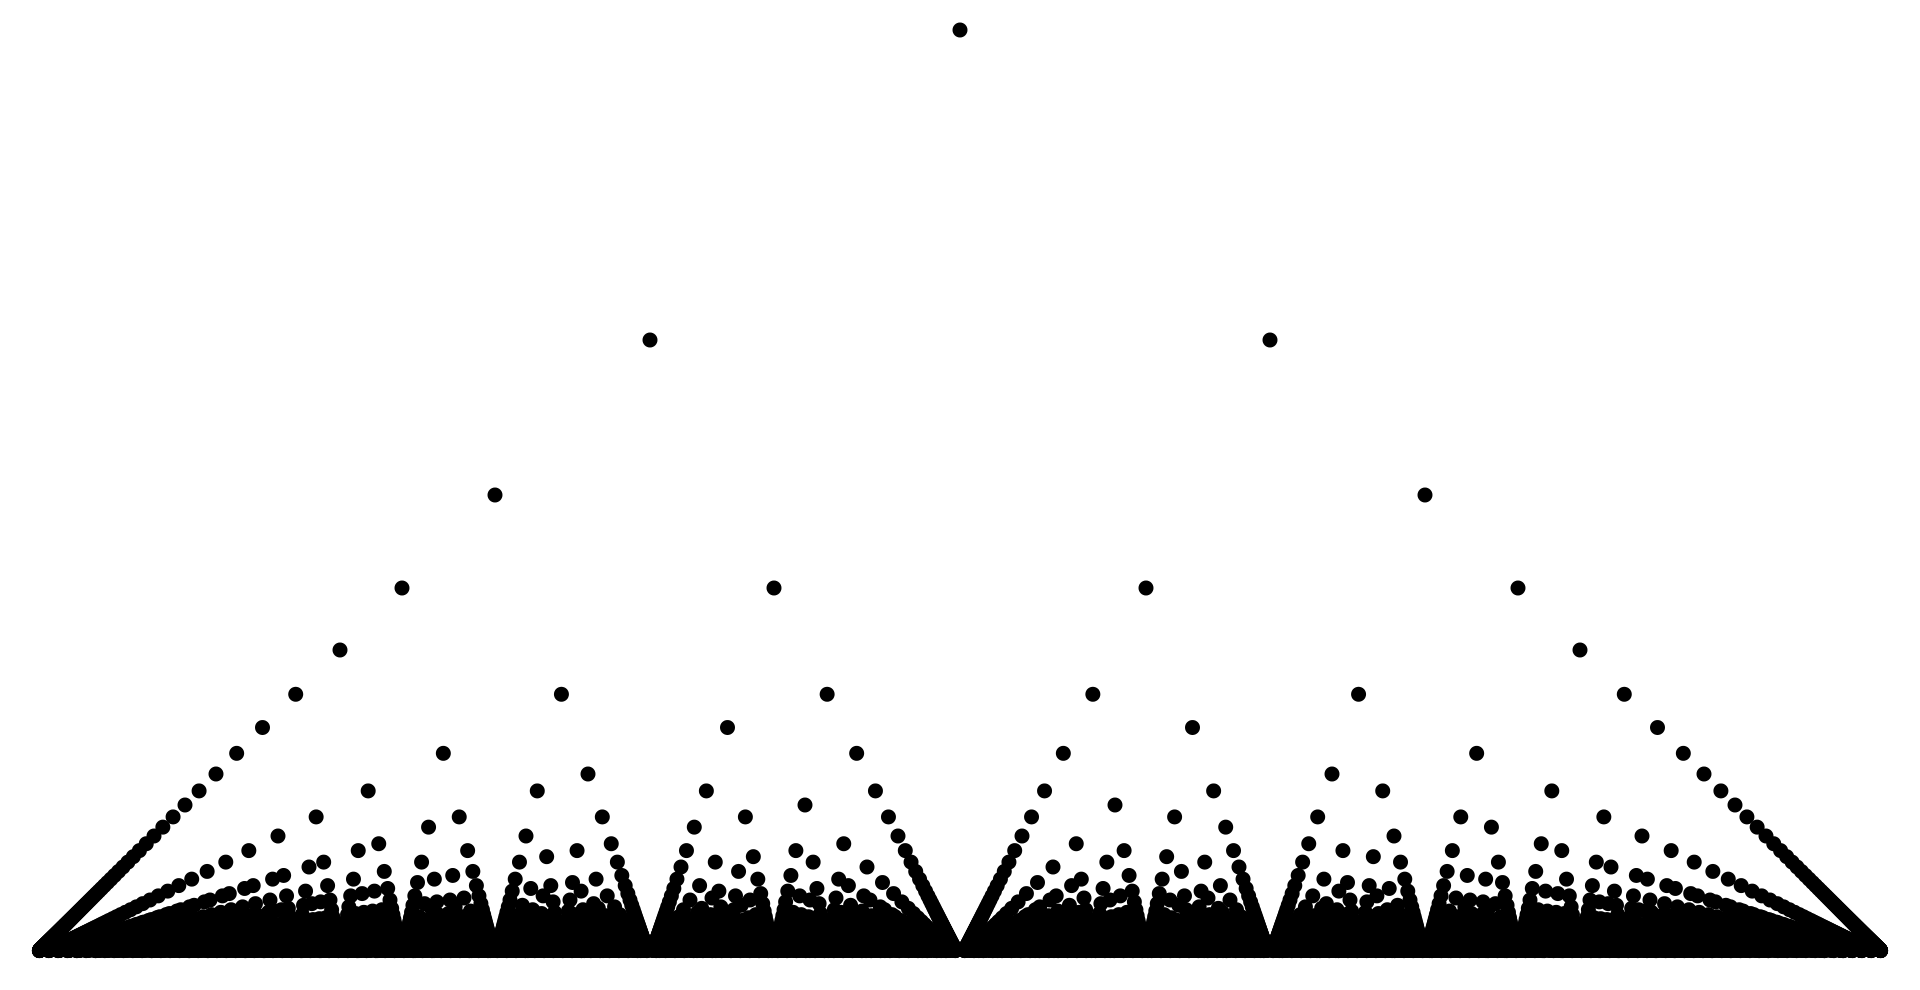
\includegraphics[width=1.\linewidth]{fig/thomae.png}
  \label{fig:thomae}
\end{figure}
\end{minipage}

\item Sutileza do domínio e contradomínio. Exemplo disso é $f:\Q \to \Q$, equação funcional $f(x+y) = f(x) + f(y)$. \textbf{Mencionar EDOs}.
\item Gráfico polar: $r(\theta) = \theta$, $r(\theta) = \cos(\theta)$ e $r(\theta) = \cos(5\theta)$.
\item Funções básicas: $x$, $x^n$, $1/x$, $e^x$, $\log(x)$, $\sin(x)$, $\abs{x}$.
\item Jogo de gráficos de funções:
\begin{itemize}
\item $x^2 + \sin(x)$, $e^{-x} \cos(x)$, $x + \frac{1}{x}, \frac{\sin(x)}{x}$, $\sqrt{1+x^2}$.
\item Jogo inverso: $(x^2 - 1)^2$, $\frac{x + \abs{x}}{2}$, $\frac{x}{\abs{x}}$.
\item Composição de funções, inversa.
\item Translações verticais e horizontais, reflexões com módulo.
\item Propriedades: paridade, periodicidade, limites para infinito, raízes, ponto fixo, derivada.
\end{itemize}
\end{itemize}


\section{Cultura}

\begin{itemize}
\item $1 + \frac{1}{2 + \frac{1}{2 + \cdots}} = \sqrt{2}$ como limite.
\item Derivada $\lim_{h \to 0} \frac{f(x+h) - f(x)}{h}$. Polinômios, trigonométricas, exponencial, log.
\item $\lim_{x \to 0} \frac{\sin(x)}{x}$, $\cos(x) = 1 - 2 \sin^2(x/2)$.
\item Exponencial
$$
e^x = \lim_{u \to \infty} \qty(1 + \frac{x}{u})^u,
$$
associada a equação $f_n(x) = \qty(1 + \frac{x}{n}) f_n'(x)$. Com isso dá para resolver $m \dot{v} = -k v$.
\item Mapa logístico, $f(x) = x$ e $f(f(x)) = x$.
\item Integral $\int_0^b x^2 \dd{x}$ usando $1^2 + 2^2 + \ldots + n^2 = f(n)$, com $f(x) = ax^3 + bx^2 + cx + d$.
\end{itemize}


\end{document}
